\documentclass[a4paper]{article}
%\usepackage{fixltx2e} % LaTeX patches, \textsubscript
%\usepackage{cmap} % fix search and cut-and-paste in Acrobat
\usepackage[T1]{fontenc}
\usepackage[utf8]{inputenc}
\usepackage{amsmath}
\usepackage{graphicx}
\usepackage{mathptmx} % Times
\usepackage[scaled=.90]{helvet}
\usepackage{courier}
\usepackage[margin=0.5in]{geometry}
\usepackage{xcolor}
\usepackage{longtable}
%%% User specified packages and stylesheets
\DeclareGraphicsExtensions{ %
    .pdf,.PDF,%
    .png,.PNG,%
    .jpg,.mps,.jpeg,.jbig2,.jb2,.JPG,.JPEG,.JBIG2,.JB2}
\title{PyRETIS --- RETIS analysis}
\author{}
\date{}

\begin{document}
\maketitle
\noindent RETIS analysis report generated by PyRETIS version 3.0.1
on 22.05.2026 13:38:58.
\\
\noindent The main results are:
\begin{itemize}
\item The crossing probability:
$P_{\text{cross}} =$ \colorbox{blue!30}{ $5.338874861 \times 10^{-4}$ }  $\pm$ $19.490487274$ $\%$

\item The initial flux (unit: 1/gromacs):
$f_A =$ \colorbox{blue!30}{ $13.363346948$ }  $\pm$ $2.727568203$ $\%$

\item The rate constant (unit: 1/gromacs):
$k_{AB} = $ \colorbox{blue!30}{ $7.134523708 \times 10^{-3}$ }  $\pm$ $19.680414693$ $\%$



\end{itemize}
\noindent Detailed results are given below for the different path
ensembles and the overall results are summarized
in the last section.

\begin{center}




\end{center}


\section{Combined results}
\label{sec:combined}

The overall matched probability distributions are shown in the left figure
while the matched probability distribution is shown in the right figure below.
The overall crossing rate as a function of cycles
and its relative error block analysis are reported in the two following
plots, respectively.

\begin{center}
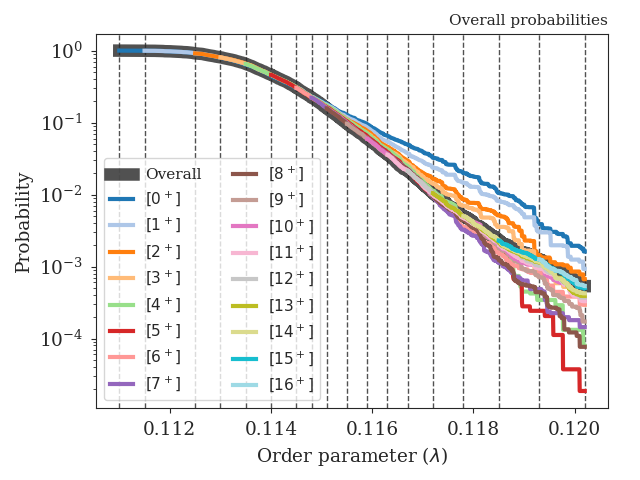
\includegraphics[width=0.45\linewidth]{total-probability.png}%
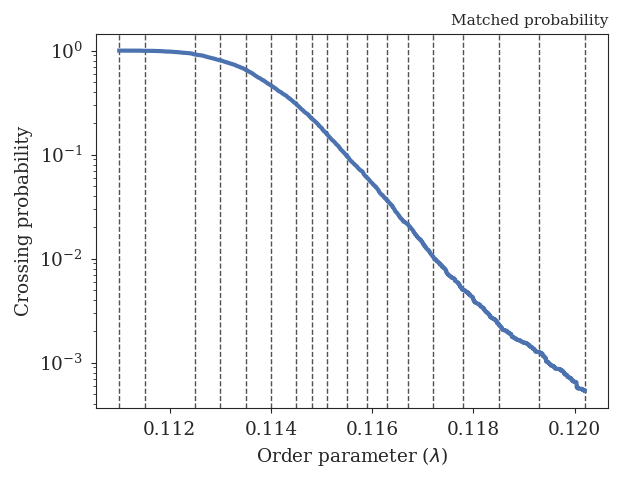
\includegraphics[width=0.45\linewidth]{matched-probability.png}%
\end{center}
\begin{center}
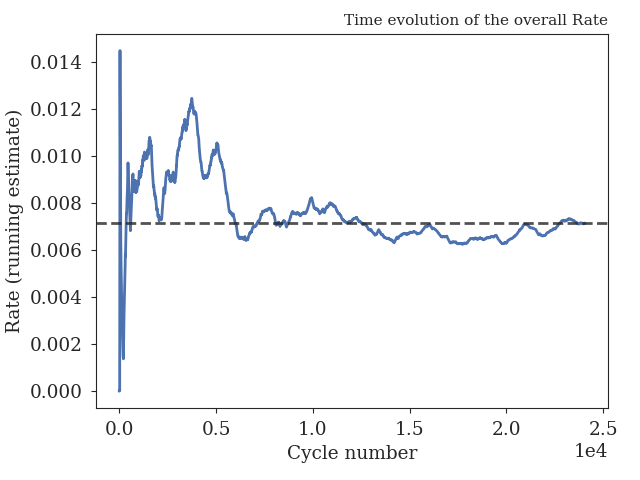
\includegraphics[width=0.45\linewidth]{overall-rrun.png}%
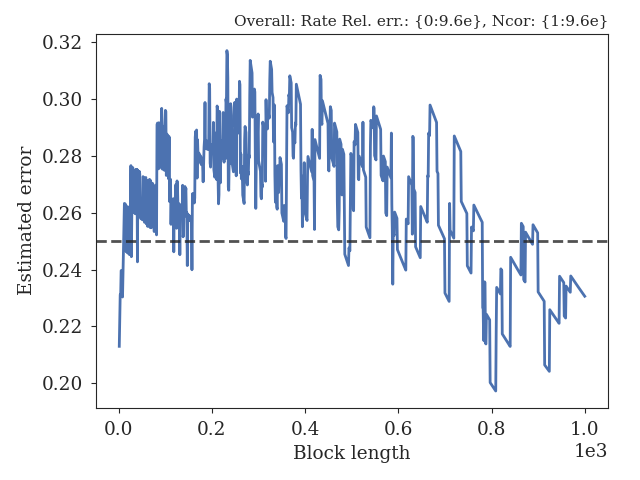
\includegraphics[width=0.45\linewidth]{overall-err.png}%
\end{center}

\clearpage

\section{Results for path ensembles}
The following interfaces were used in the simulation and in
the analysis:
\begin{longtable}{| c | c | c | c |}
\caption{Interfaces}\\
\hline
Ensemble & Left & Middle & Detect\\ \hline
$ [0^-]  $ & $  -inf  $ & $ 0.1110 $ & $$\\
$ [0^+]  $ & $ 0.1110 $ & $ 0.1110 $ & $ 0.1115 $\\
$ [1^+]  $ & $ 0.1110 $ & $ 0.1115 $ & $ 0.1125 $\\
$ [2^+]  $ & $ 0.1110 $ & $ 0.1125 $ & $ 0.1130 $\\
$ [3^+]  $ & $ 0.1110 $ & $ 0.1130 $ & $ 0.1135 $\\
$ [4^+]  $ & $ 0.1110 $ & $ 0.1135 $ & $ 0.1140 $\\
$ [5^+]  $ & $ 0.1110 $ & $ 0.1140 $ & $ 0.1145 $\\
$ [6^+]  $ & $ 0.1110 $ & $ 0.1145 $ & $ 0.1148 $\\
$ [7^+]  $ & $ 0.1110 $ & $ 0.1148 $ & $ 0.1151 $\\
$ [8^+]  $ & $ 0.1110 $ & $ 0.1151 $ & $ 0.1155 $\\
$ [9^+]  $ & $ 0.1110 $ & $ 0.1155 $ & $ 0.1159 $\\
$ [10^+] $ & $ 0.1110 $ & $ 0.1159 $ & $ 0.1163 $\\
$ [11^+] $ & $ 0.1110 $ & $ 0.1163 $ & $ 0.1167 $\\
$ [12^+] $ & $ 0.1110 $ & $ 0.1167 $ & $ 0.1172 $\\
$ [13^+] $ & $ 0.1110 $ & $ 0.1172 $ & $ 0.1178 $\\
$ [14^+] $ & $ 0.1110 $ & $ 0.1178 $ & $ 0.1185 $\\
$ [15^+] $ & $ 0.1110 $ & $ 0.1185 $ & $ 0.1193 $\\
$ [16^+] $ & $ 0.1110 $ & $ 0.1193 $ & $ 0.1202 $\\
\hline
\end{longtable}
\begin{longtable}{| c | c | c | c |}
\caption{Crossing probabilities}\\
\hline
Ensemble & $P_\text{cross}$ & Error & Rel. error (\%)\\ \hline
$ [0^+]  $ & $ 0.995875 $ & $ 0.001968 $ & $ 0.197593 $\\
$ [1^+]  $ & $ 0.919191 $ & $ 0.007091 $ & $ 0.771398 $\\
$ [2^+]  $ & $ 0.880445 $ & $ 0.007888 $ & $ 0.895898 $\\
$ [3^+]  $ & $ 0.809343 $ & $ 0.009357 $ & $ 1.156072 $\\
$ [4^+]  $ & $ 0.707217 $ & $ 0.010096 $ & $ 1.427504 $\\
$ [5^+]  $ & $ 0.661355 $ & $ 0.012037 $ & $ 1.819992 $\\
$ [6^+]  $ & $ 0.727769 $ & $ 0.014310 $ & $ 1.966314 $\\
$ [7^+]  $ & $ 0.711102 $ & $ 0.013358 $ & $ 1.878497 $\\
$ [8^+]  $ & $ 0.611956 $ & $ 0.019939 $ & $ 3.258187 $\\
$ [9^+]  $ & $ 0.617765 $ & $ 0.020314 $ & $ 3.288292 $\\
$ [10^+] $ & $ 0.600065 $ & $ 0.023338 $ & $ 3.889320 $\\
$ [11^+] $ & $ 0.598512 $ & $ 0.021873 $ & $ 3.654527 $\\
$ [12^+] $ & $ 0.488019 $ & $ 0.029900 $ & $ 6.126788 $\\
$ [13^+] $ & $ 0.477673 $ & $ 0.033546 $ & $ 7.022869 $\\
$ [14^+] $ & $ 0.460242 $ & $ 0.040909 $ & $ 8.888646 $\\
$ [15^+] $ & $ 0.549635 $ & $ 0.037555 $ & $ 6.832631 $\\
$ [16^+] $ & $ 0.422327 $ & $ 0.042632 $ & $10.094477 $\\
\hline
\end{longtable}
\begin{longtable}{| c | c | c | c | c |}
\caption{Pathensemble data}\\
\hline
Ensemble & TIS cycles & Shoot acc. ratio & Swap acc. ratio & Avg. path length\\ \hline
$ [0^-]  $ & $  24640   $ & $ 0.832947 $ & $ 0.211561 $ & $ 3.000162 $\\
$ [0^+]  $ & $  24725   $ & $ 0.675111 $ & $ 0.608892 $ & $ 8.482993 $\\
$ [1^+]  $ & $  24725   $ & $ 0.685823 $ & $ 0.958105 $ & $ 8.822568 $\\
$ [2^+]  $ & $  24725   $ & $ 0.693767 $ & $ 0.896836 $ & $ 9.419171 $\\
$ [3^+]  $ & $  24725   $ & $ 0.685256 $ & $ 0.838715 $ & $10.144590 $\\
$ [4^+]  $ & $  24718   $ & $ 0.671396 $ & $ 0.754522 $ & $11.458209 $\\
$ [5^+]  $ & $  24725   $ & $ 0.651131 $ & $ 0.682677 $ & $13.797492 $\\
$ [6^+]  $ & $  24718   $ & $ 0.635155 $ & $ 0.694687 $ & $17.239542 $\\
$ [7^+]  $ & $  24680   $ & $ 0.613092 $ & $ 0.721113 $ & $19.550527 $\\
$ [8^+]  $ & $  24724   $ & $ 0.594439 $ & $ 0.657007 $ & $23.944629 $\\
$ [9^+]  $ & $  24723   $ & $ 0.575679 $ & $ 0.611479 $ & $28.906646 $\\
$ [10^+] $ & $  24669   $ & $ 0.560332 $ & $ 0.605646 $ & $35.559852 $\\
$ [11^+] $ & $  24723   $ & $ 0.546088 $ & $ 0.596464 $ & $38.457267 $\\
$ [12^+] $ & $  24665   $ & $ 0.532347 $ & $ 0.544778 $ & $44.577458 $\\
$ [13^+] $ & $  24634   $ & $ 0.517124 $ & $ 0.480755 $ & $50.269262 $\\
$ [14^+] $ & $  24687   $ & $ 0.484005 $ & $ 0.466090 $ & $51.828007 $\\
$ [15^+] $ & $  24660   $ & $ 0.413429 $ & $ 0.506554 $ & $63.941079 $\\
$ [16^+] $ & $  24043   $ & $ 0.538006 $ & $ 0.541311 $ & $69.159381 $\\
\hline
\end{longtable}
\clearpage


\subsection{Crossing probabilities}

\begin{center}
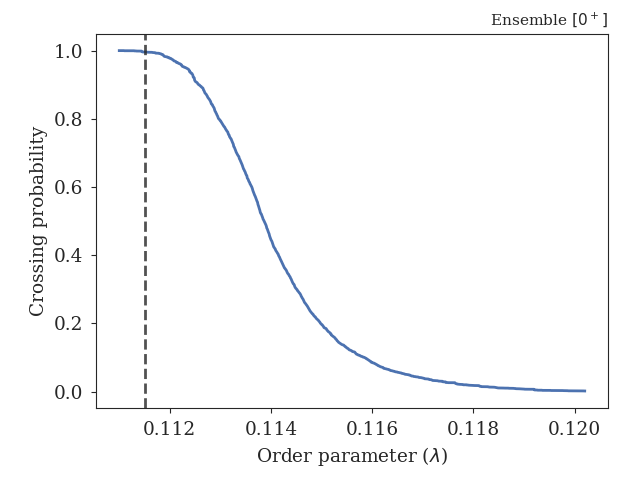
\includegraphics[width=0.33\linewidth]{001_pcross.png}%
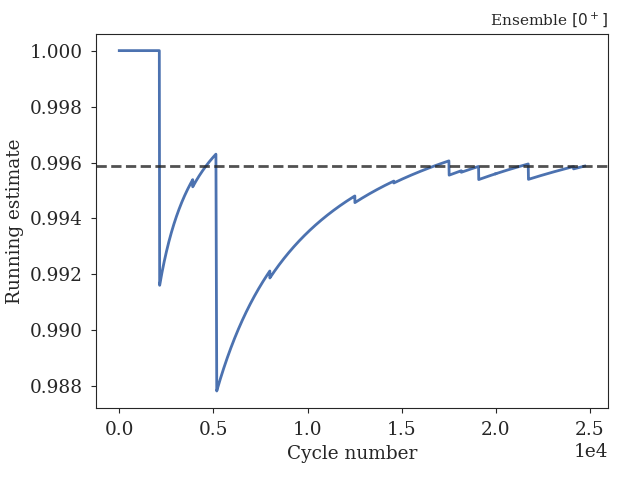
\includegraphics[width=0.33\linewidth]{001_prun.png}%
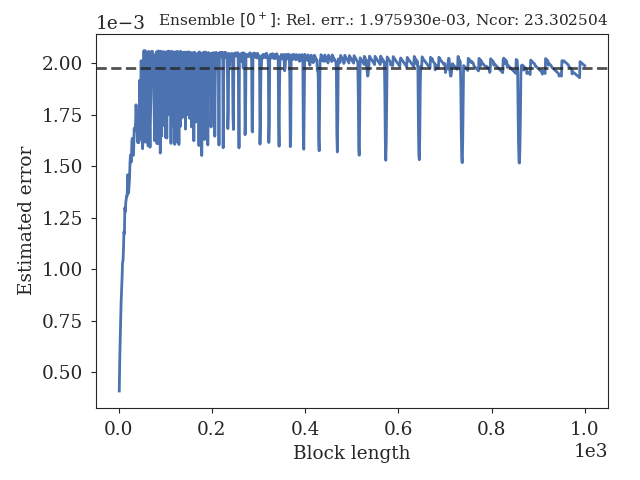
\includegraphics[width=0.33\linewidth]{001_perror.png}%
\end{center}

\begin{center}
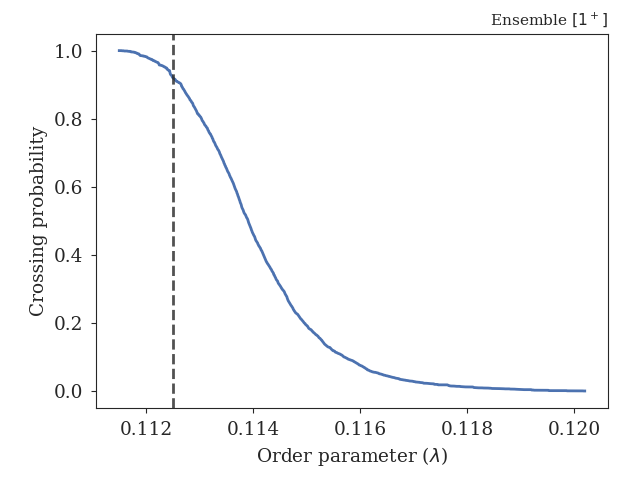
\includegraphics[width=0.33\linewidth]{002_pcross.png}%
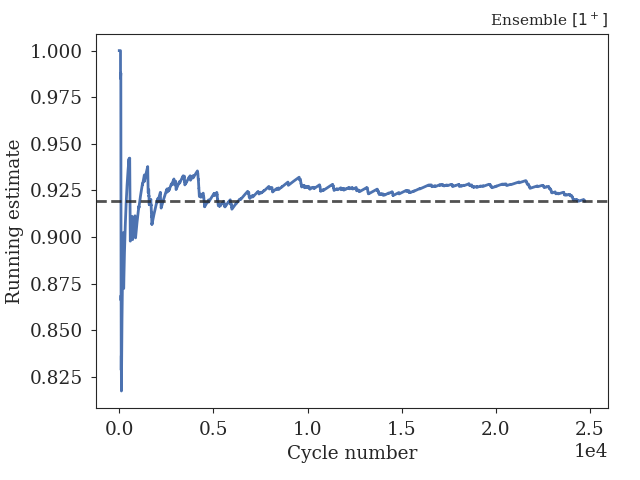
\includegraphics[width=0.33\linewidth]{002_prun.png}%
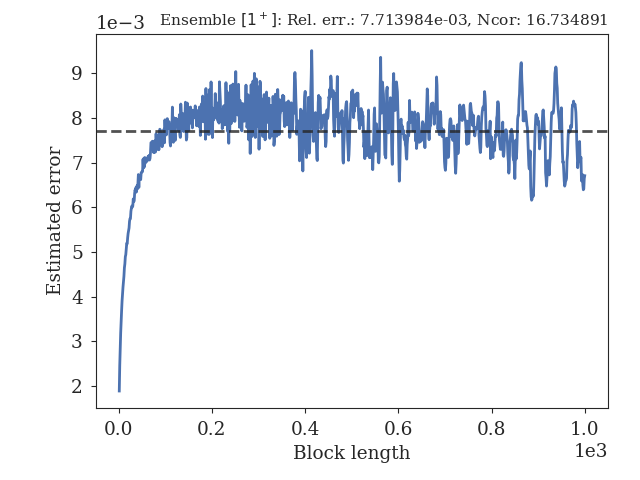
\includegraphics[width=0.33\linewidth]{002_perror.png}%
\end{center}

\begin{center}
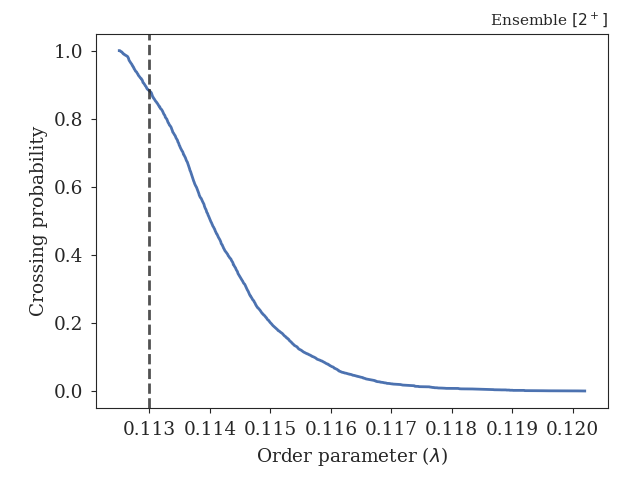
\includegraphics[width=0.33\linewidth]{003_pcross.png}%
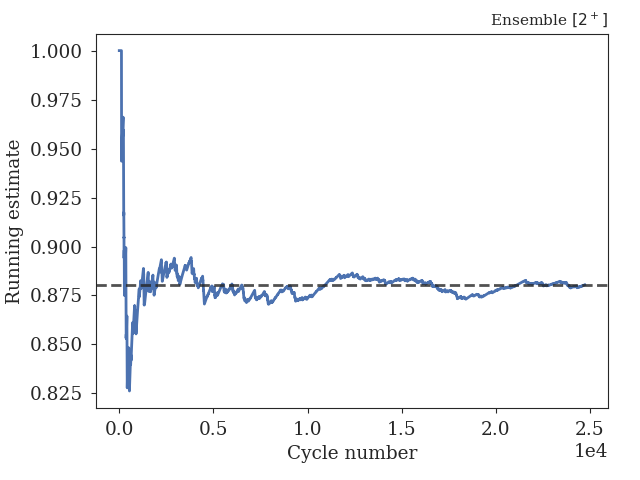
\includegraphics[width=0.33\linewidth]{003_prun.png}%
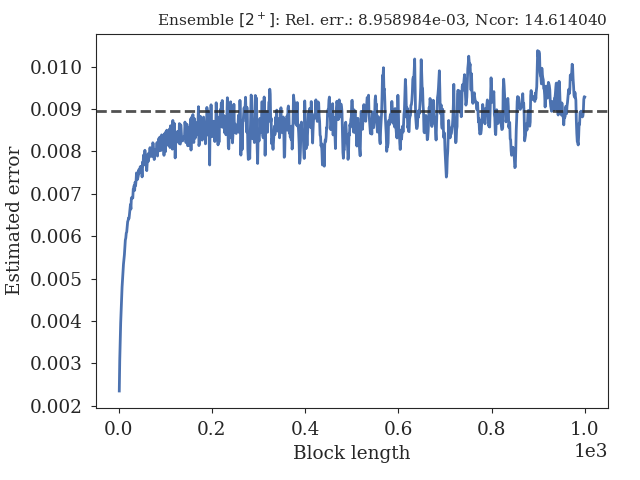
\includegraphics[width=0.33\linewidth]{003_perror.png}%
\end{center}

\begin{center}
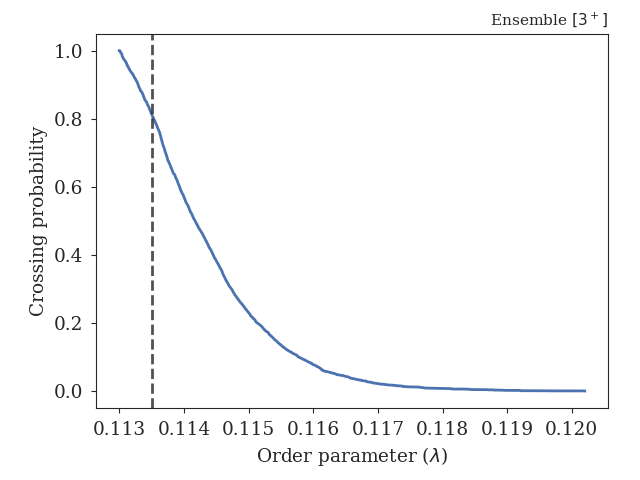
\includegraphics[width=0.33\linewidth]{004_pcross.png}%
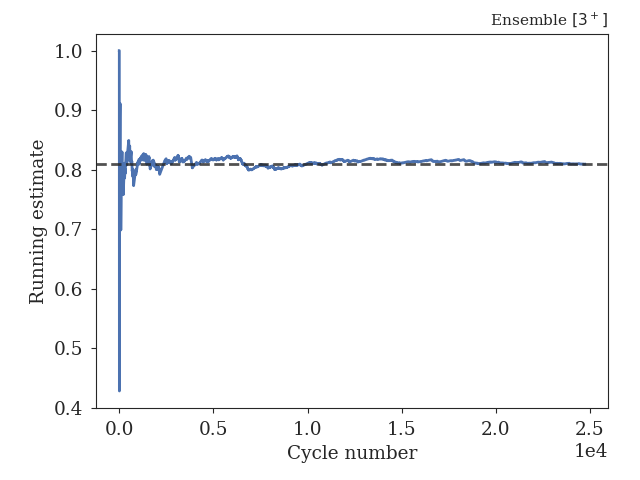
\includegraphics[width=0.33\linewidth]{004_prun.png}%
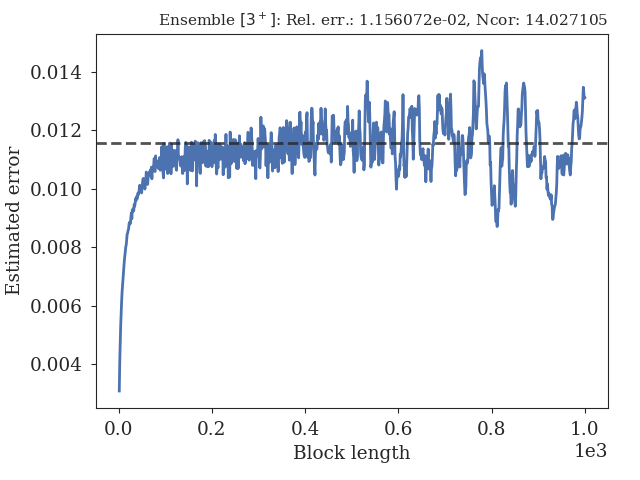
\includegraphics[width=0.33\linewidth]{004_perror.png}%
\end{center}

\begin{center}
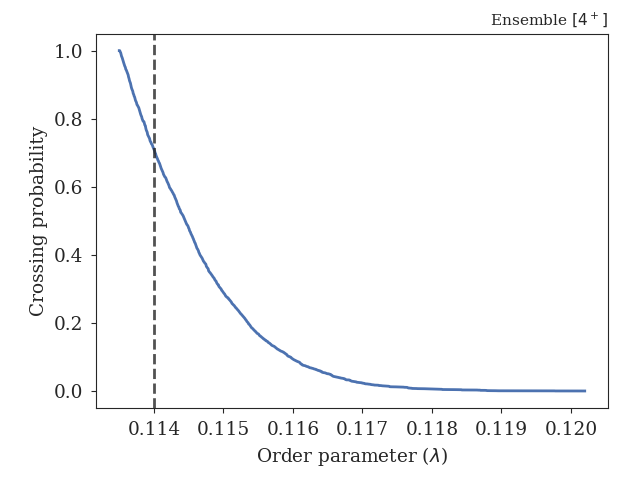
\includegraphics[width=0.33\linewidth]{005_pcross.png}%
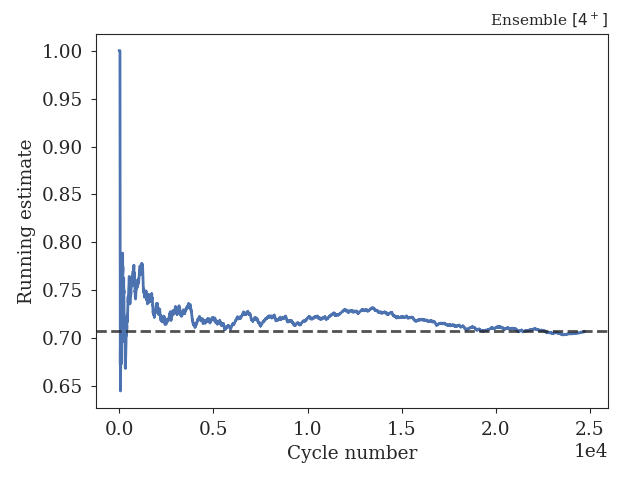
\includegraphics[width=0.33\linewidth]{005_prun.png}%
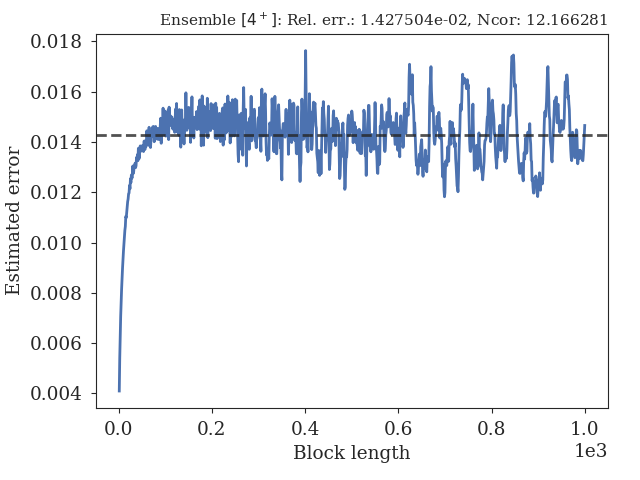
\includegraphics[width=0.33\linewidth]{005_perror.png}%
\end{center}

\begin{center}
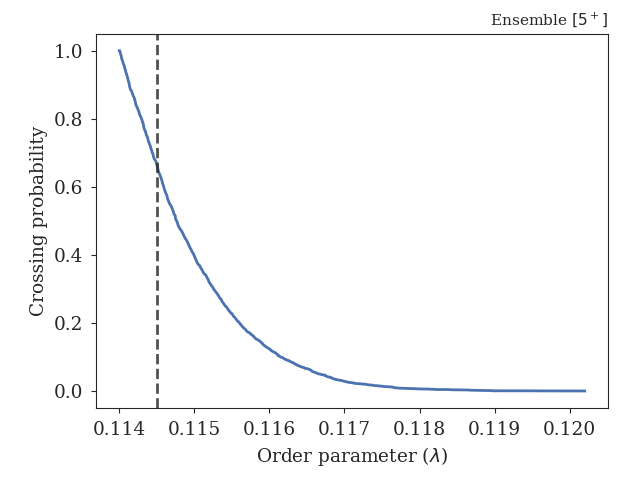
\includegraphics[width=0.33\linewidth]{006_pcross.png}%
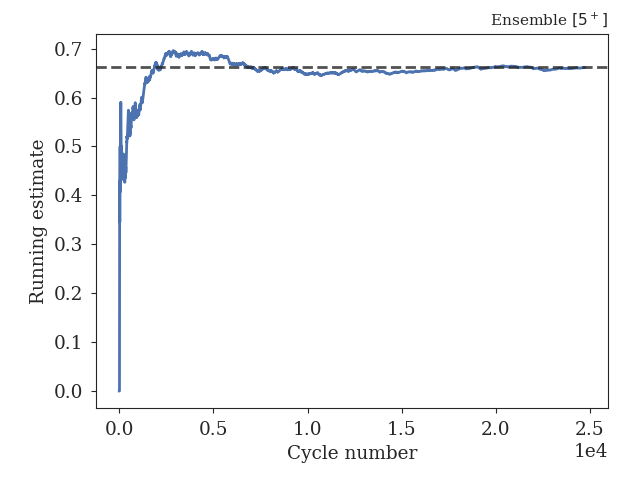
\includegraphics[width=0.33\linewidth]{006_prun.png}%
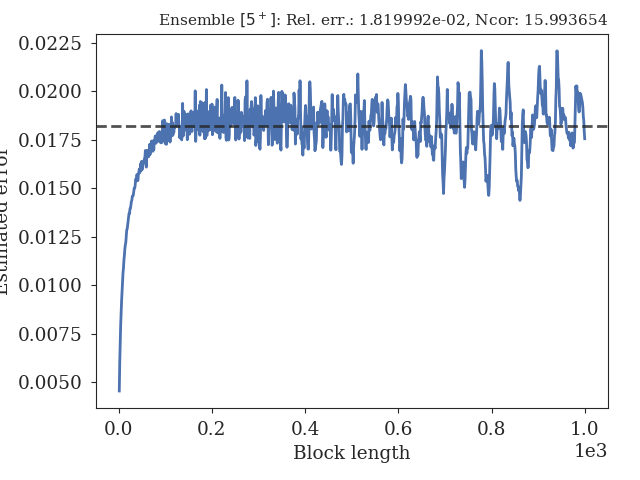
\includegraphics[width=0.33\linewidth]{006_perror.png}%
\end{center}

\begin{center}
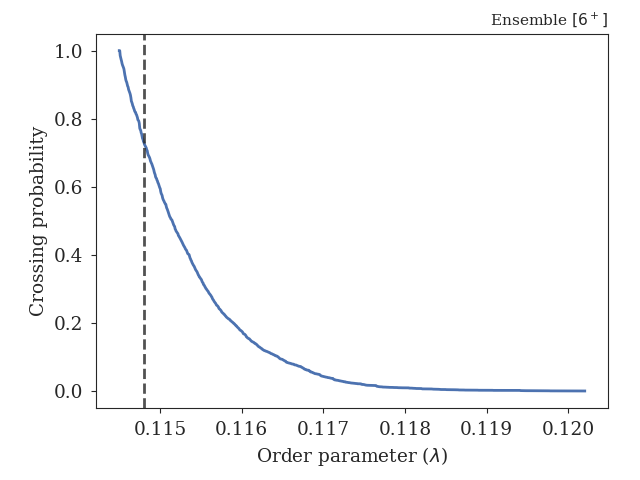
\includegraphics[width=0.33\linewidth]{007_pcross.png}%
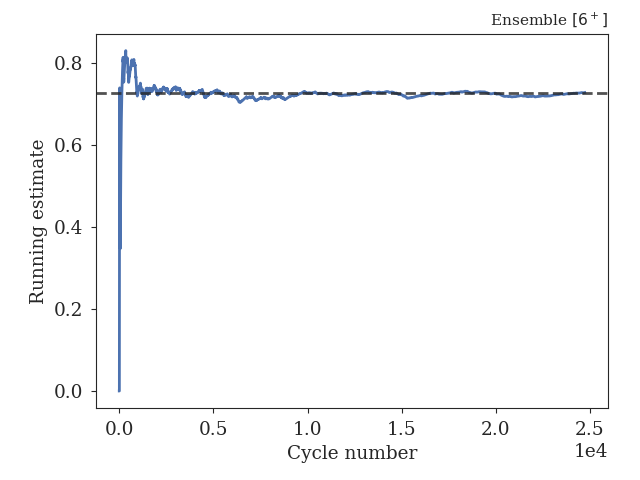
\includegraphics[width=0.33\linewidth]{007_prun.png}%
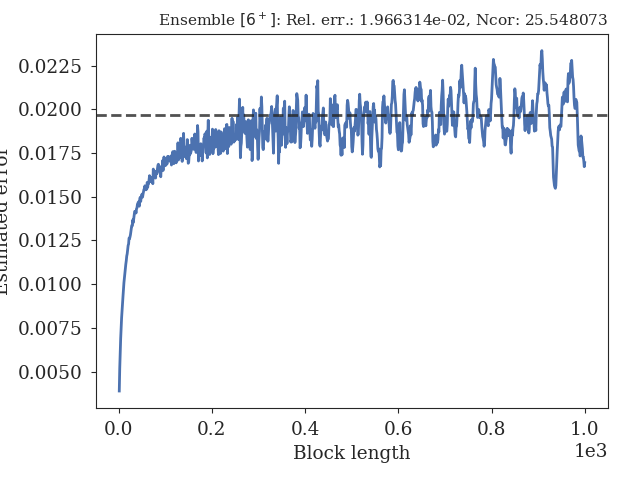
\includegraphics[width=0.33\linewidth]{007_perror.png}%
\end{center}

\begin{center}
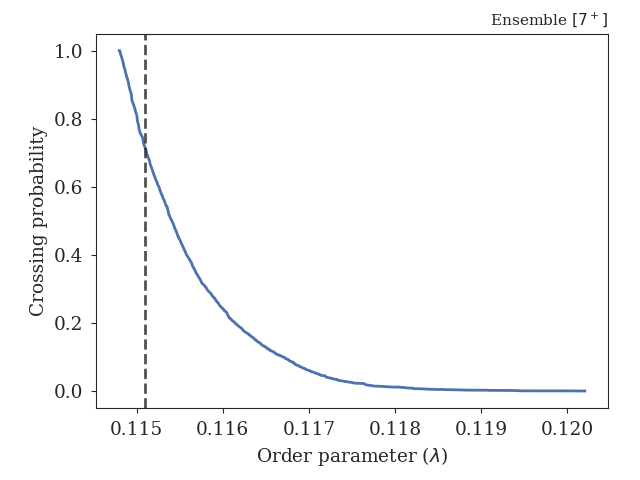
\includegraphics[width=0.33\linewidth]{008_pcross.png}%
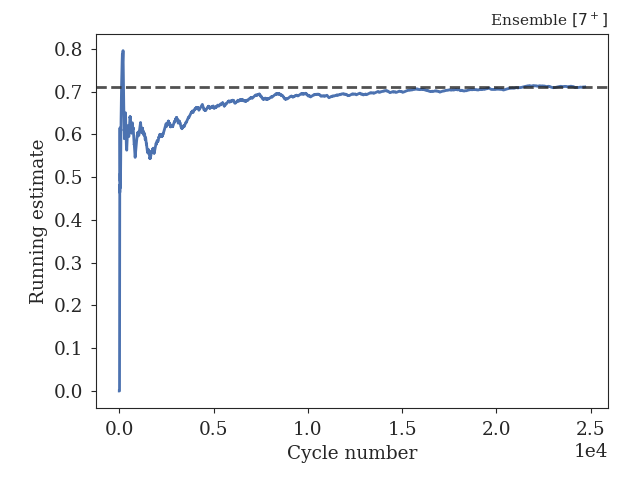
\includegraphics[width=0.33\linewidth]{008_prun.png}%
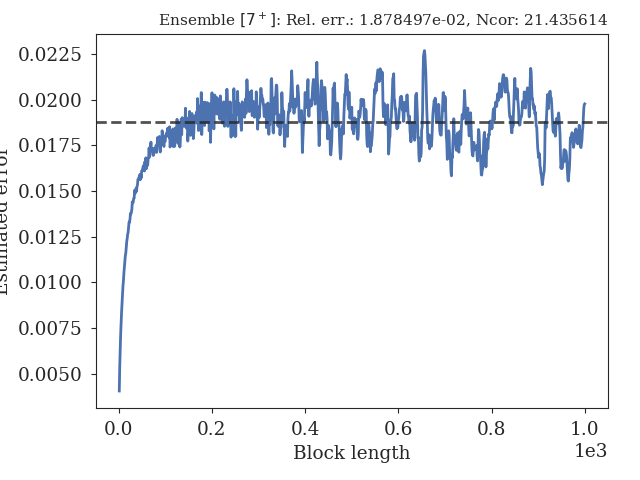
\includegraphics[width=0.33\linewidth]{008_perror.png}%
\end{center}

\begin{center}
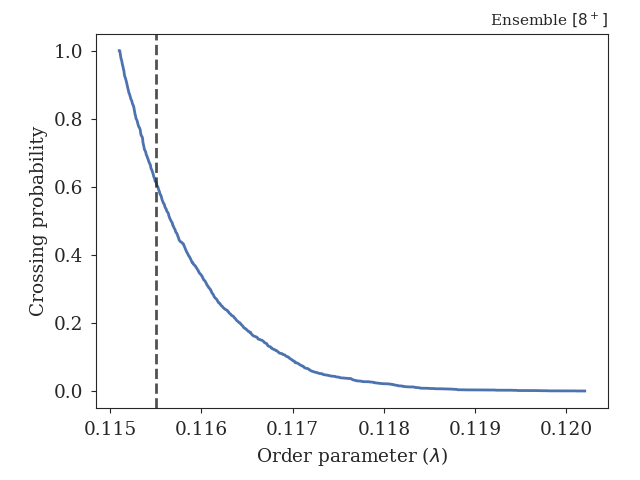
\includegraphics[width=0.33\linewidth]{009_pcross.png}%
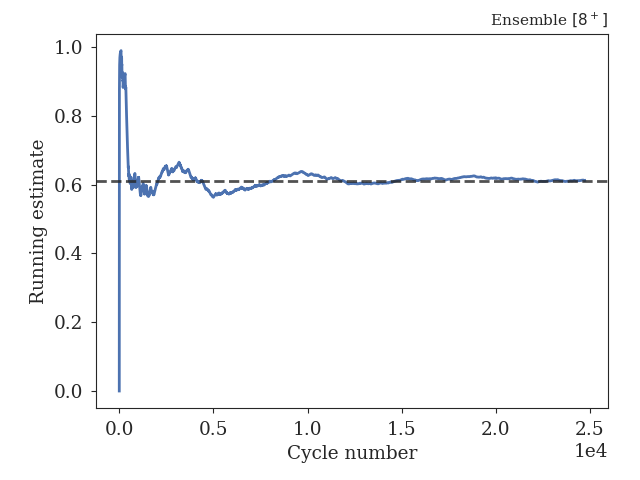
\includegraphics[width=0.33\linewidth]{009_prun.png}%
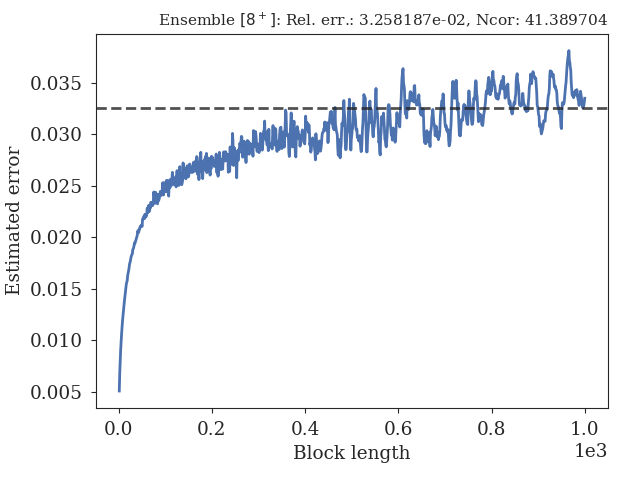
\includegraphics[width=0.33\linewidth]{009_perror.png}%
\end{center}

\begin{center}
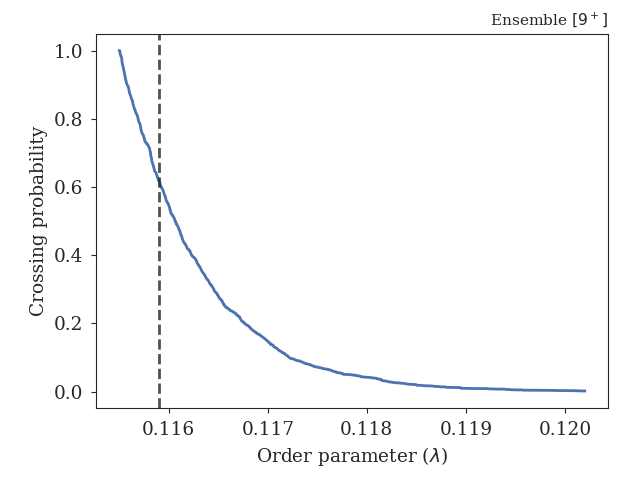
\includegraphics[width=0.33\linewidth]{010_pcross.png}%
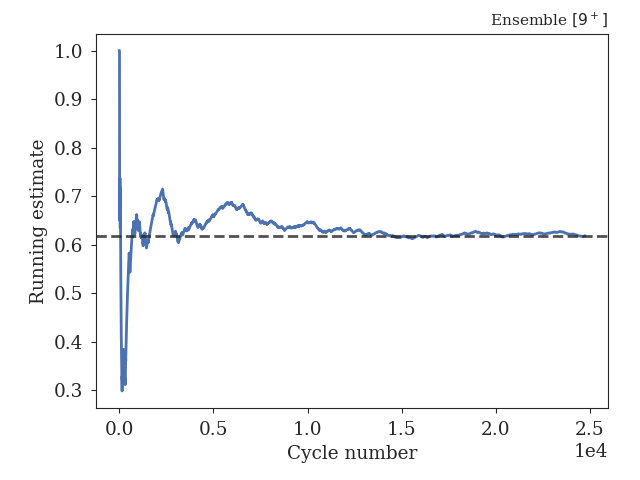
\includegraphics[width=0.33\linewidth]{010_prun.png}%
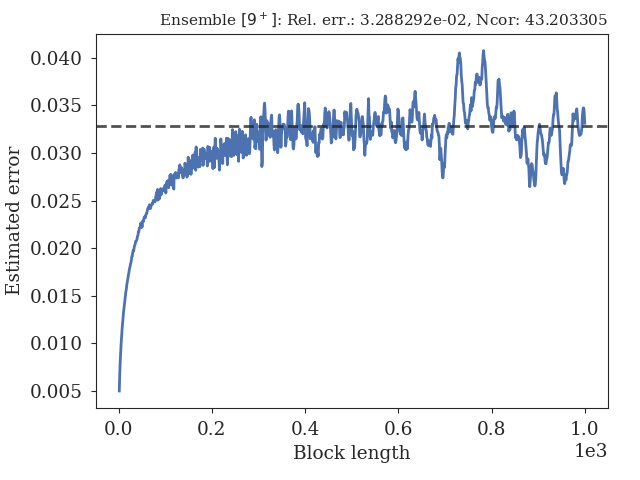
\includegraphics[width=0.33\linewidth]{010_perror.png}%
\end{center}

\begin{center}
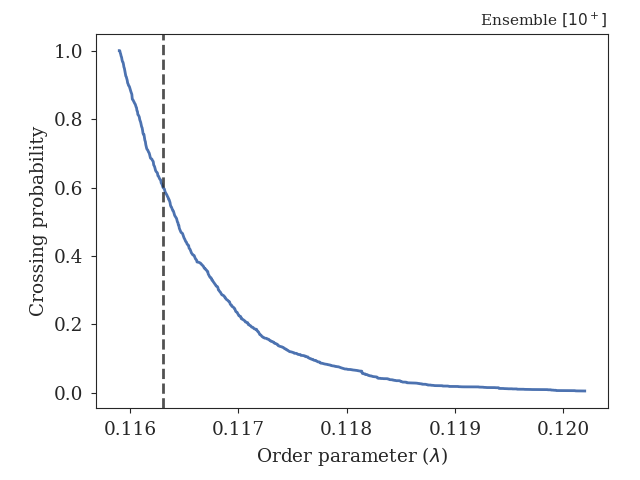
\includegraphics[width=0.33\linewidth]{011_pcross.png}%
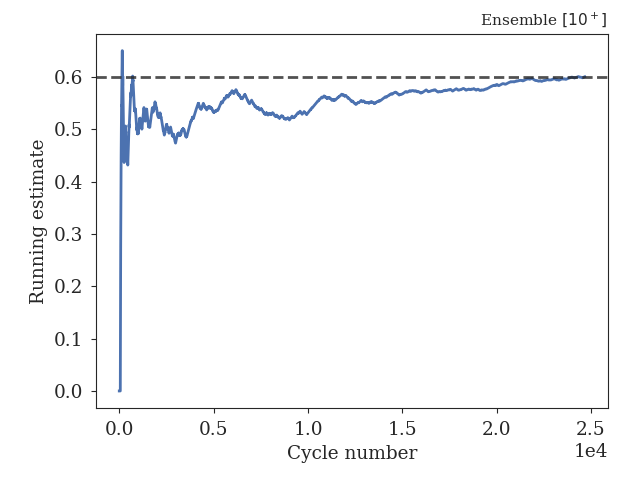
\includegraphics[width=0.33\linewidth]{011_prun.png}%
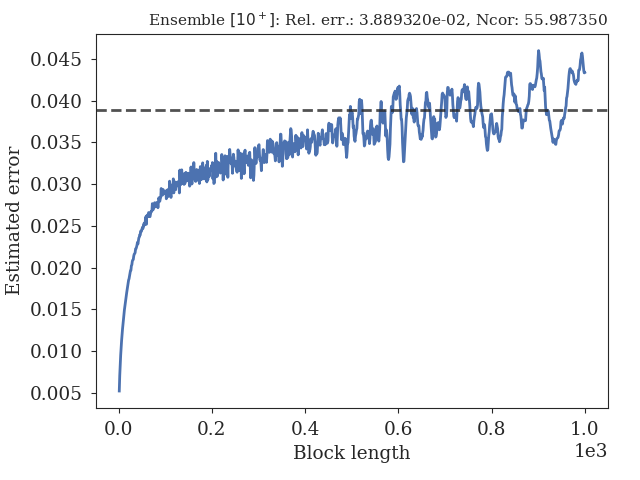
\includegraphics[width=0.33\linewidth]{011_perror.png}%
\end{center}

\begin{center}
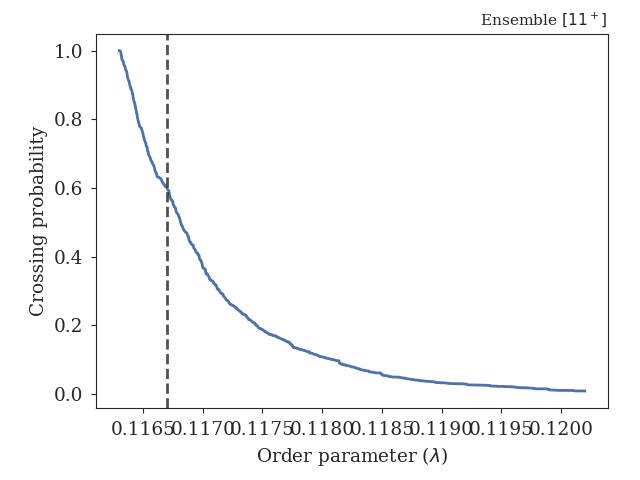
\includegraphics[width=0.33\linewidth]{012_pcross.png}%
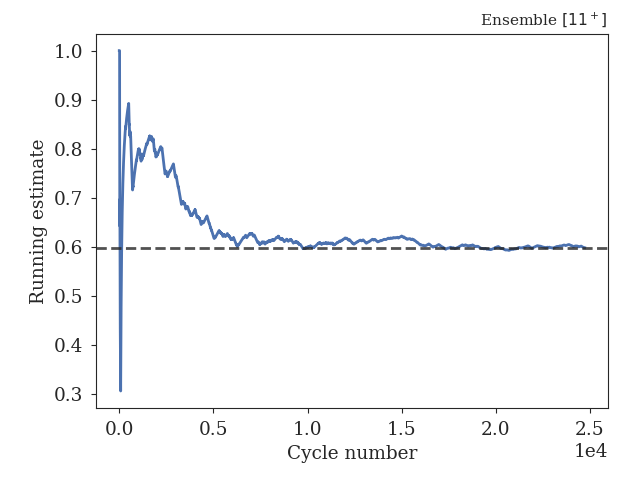
\includegraphics[width=0.33\linewidth]{012_prun.png}%
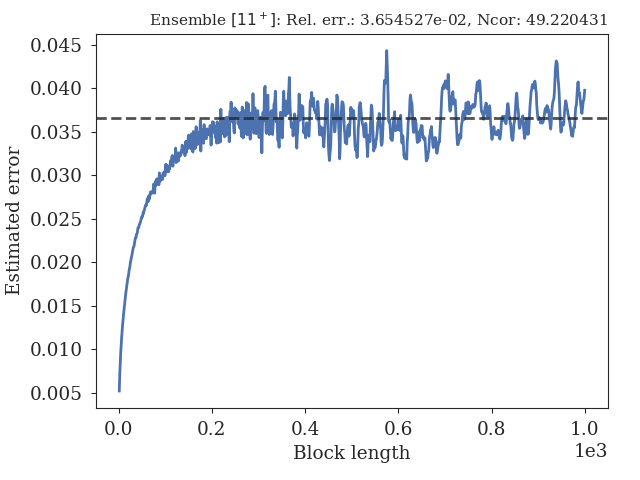
\includegraphics[width=0.33\linewidth]{012_perror.png}%
\end{center}

\begin{center}
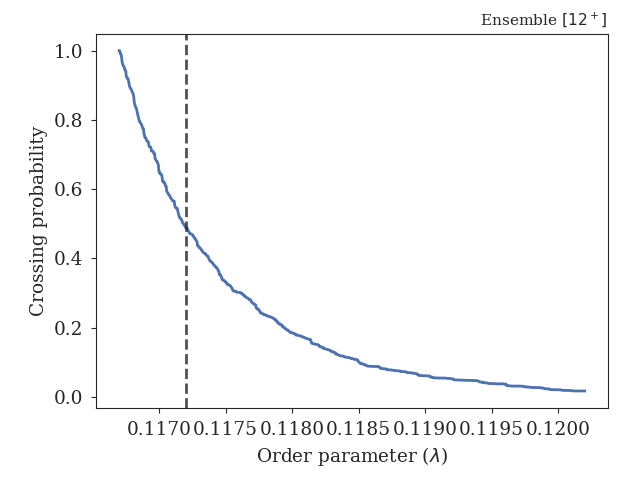
\includegraphics[width=0.33\linewidth]{013_pcross.png}%
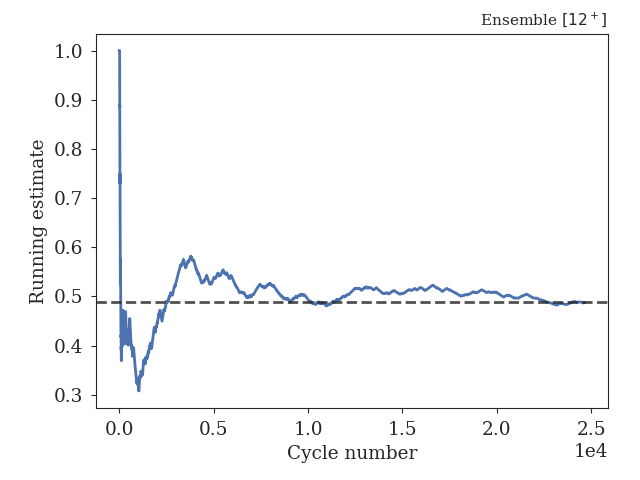
\includegraphics[width=0.33\linewidth]{013_prun.png}%
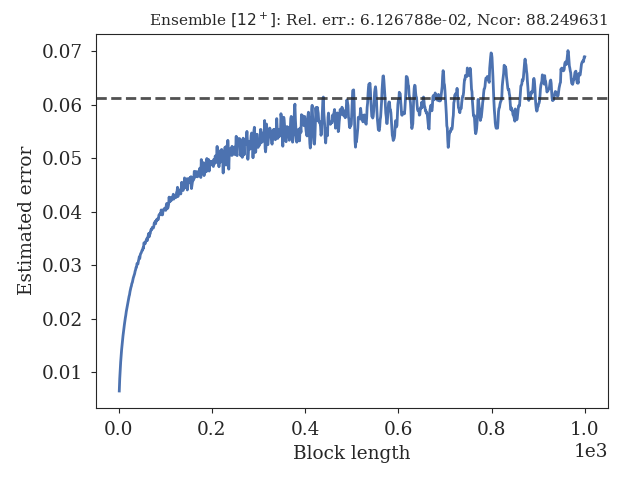
\includegraphics[width=0.33\linewidth]{013_perror.png}%
\end{center}

\begin{center}
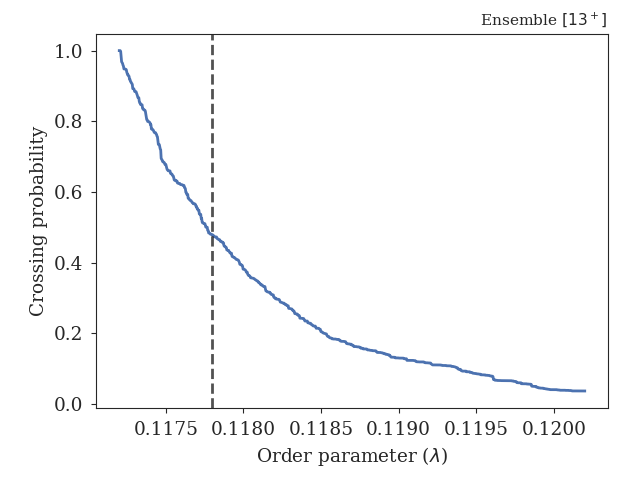
\includegraphics[width=0.33\linewidth]{014_pcross.png}%
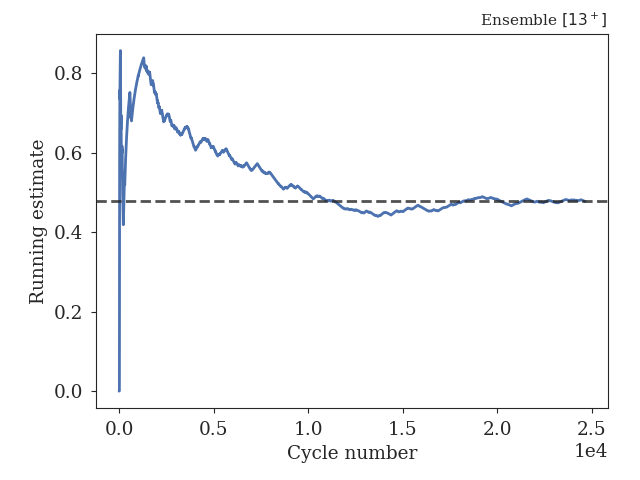
\includegraphics[width=0.33\linewidth]{014_prun.png}%
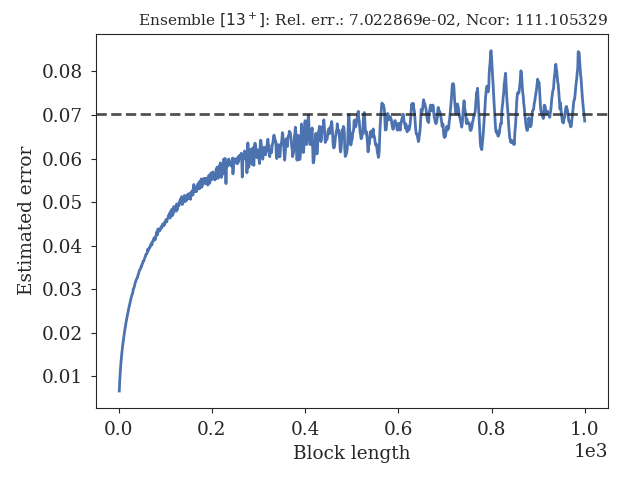
\includegraphics[width=0.33\linewidth]{014_perror.png}%
\end{center}

\begin{center}
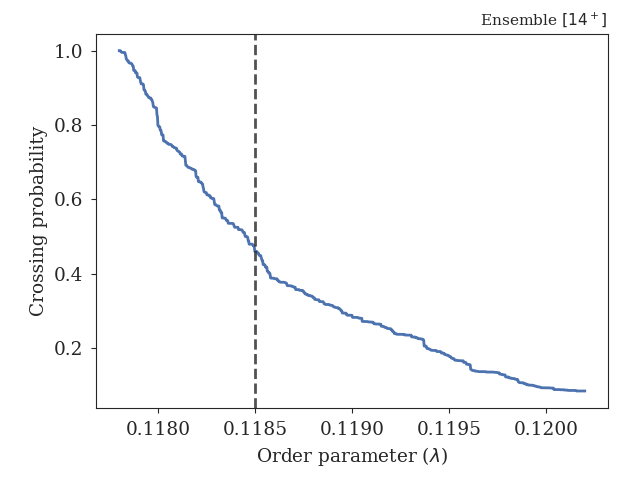
\includegraphics[width=0.33\linewidth]{015_pcross.png}%
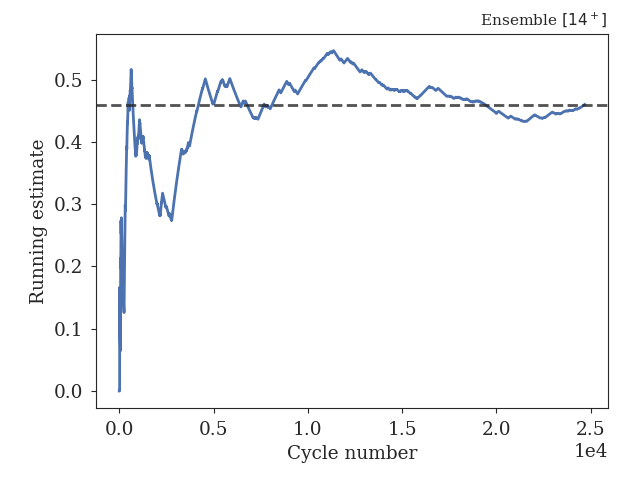
\includegraphics[width=0.33\linewidth]{015_prun.png}%
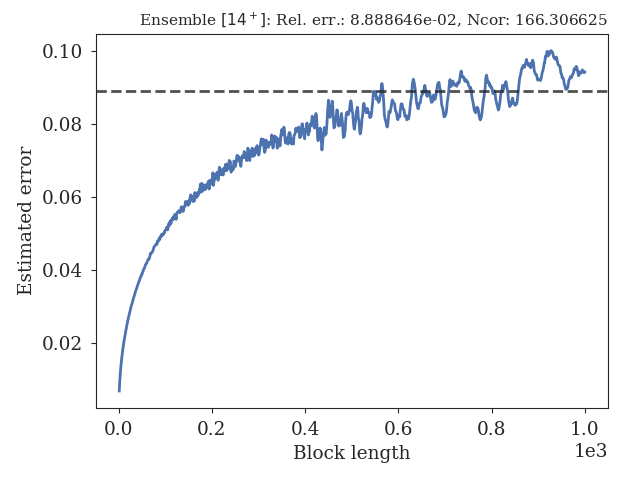
\includegraphics[width=0.33\linewidth]{015_perror.png}%
\end{center}

\begin{center}
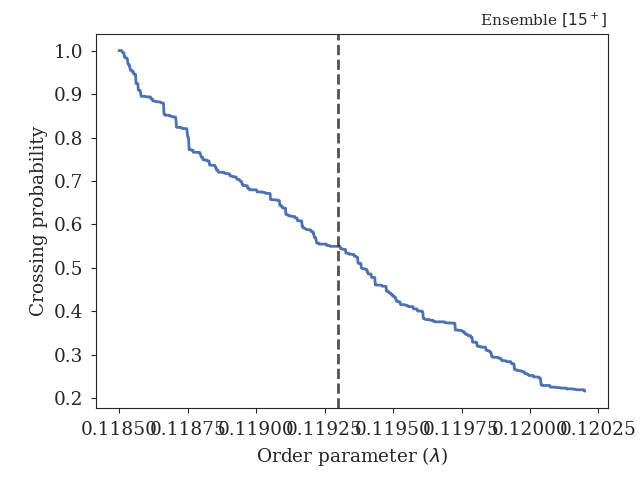
\includegraphics[width=0.33\linewidth]{016_pcross.png}%
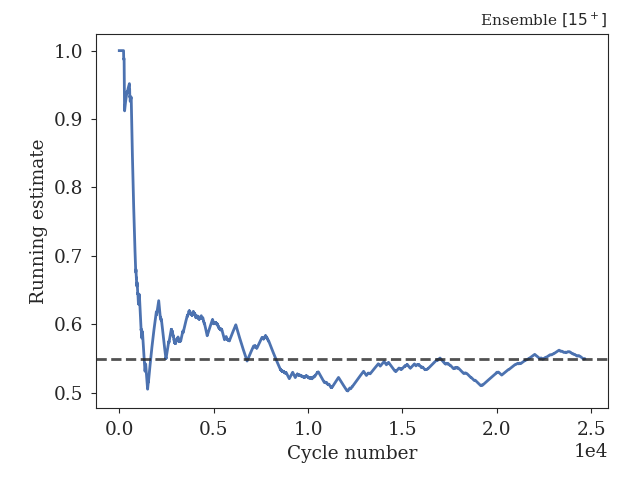
\includegraphics[width=0.33\linewidth]{016_prun.png}%
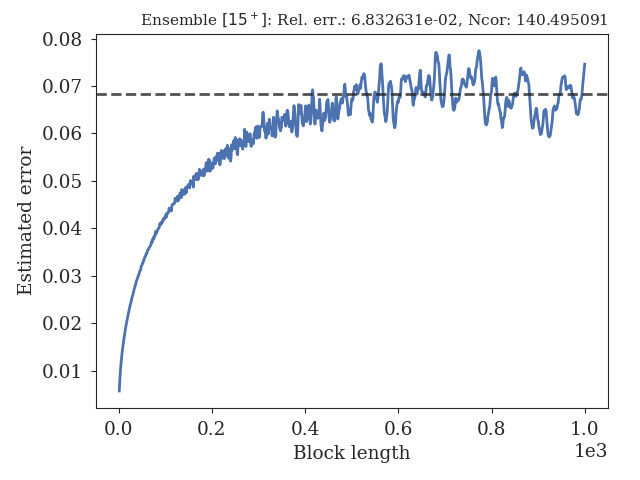
\includegraphics[width=0.33\linewidth]{016_perror.png}%
\end{center}

\begin{center}
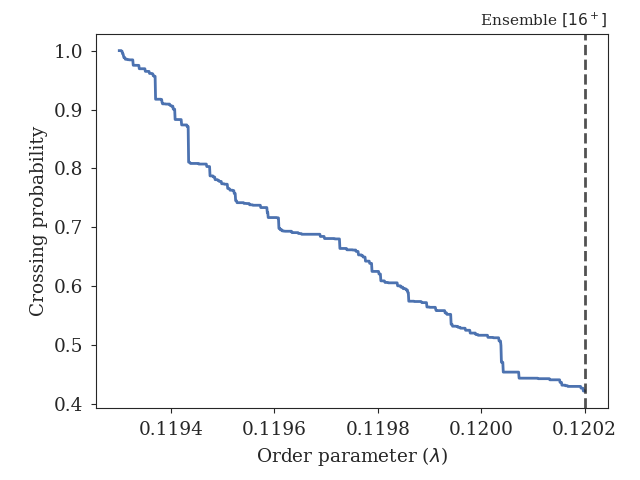
\includegraphics[width=0.33\linewidth]{017_pcross.png}%
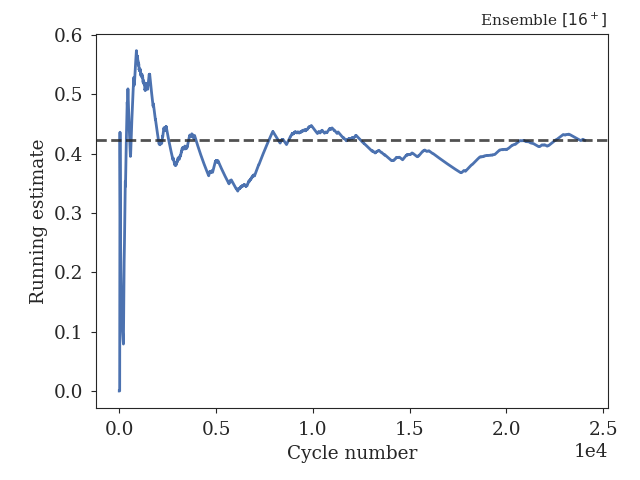
\includegraphics[width=0.33\linewidth]{017_prun.png}%
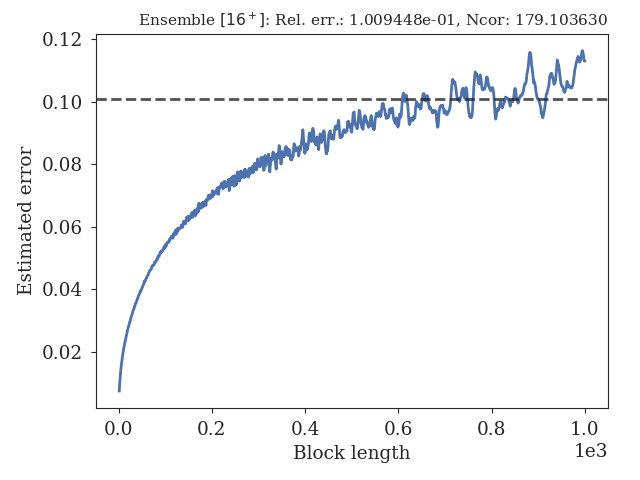
\includegraphics[width=0.33\linewidth]{017_perror.png}%
\end{center}

\clearpage

\subsection{Distributions for path lengths and shooting moves}
The average path lengths in the different ensembles are given in
the table below and some distributions for the path lengths and
shooting moves can also be found here:

\begin{center}

\includegraphics[width=0.45\linewidth]{000_lpath.png}%

\includegraphics[width=0.45\linewidth]{000_shoots.png}%
\end{center}


\begin{center}
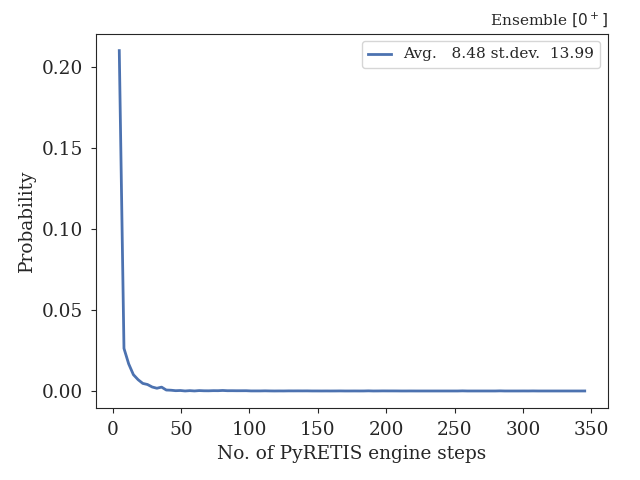
\includegraphics[width=0.45\linewidth]{001_lpath.png}%
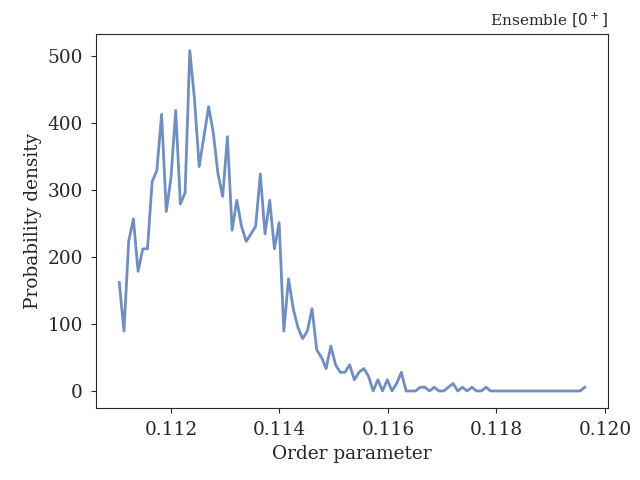
\includegraphics[width=0.45\linewidth]{001_shoots.png}%
\end{center}

\begin{center}
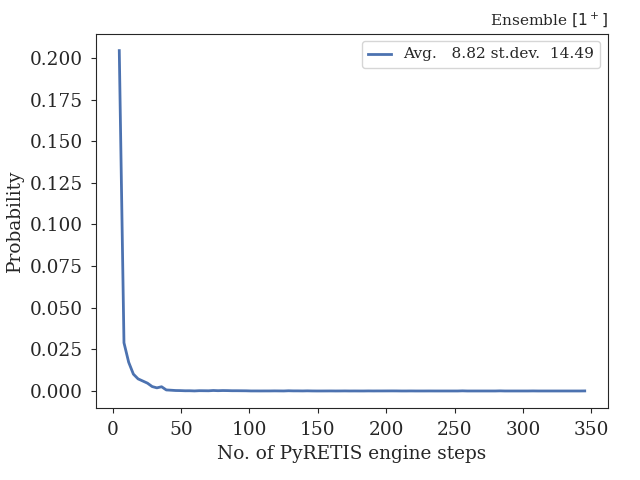
\includegraphics[width=0.45\linewidth]{002_lpath.png}%
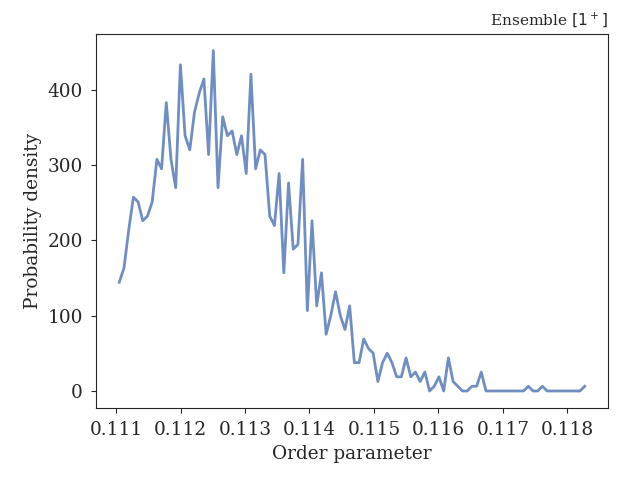
\includegraphics[width=0.45\linewidth]{002_shoots.png}%
\end{center}

\begin{center}
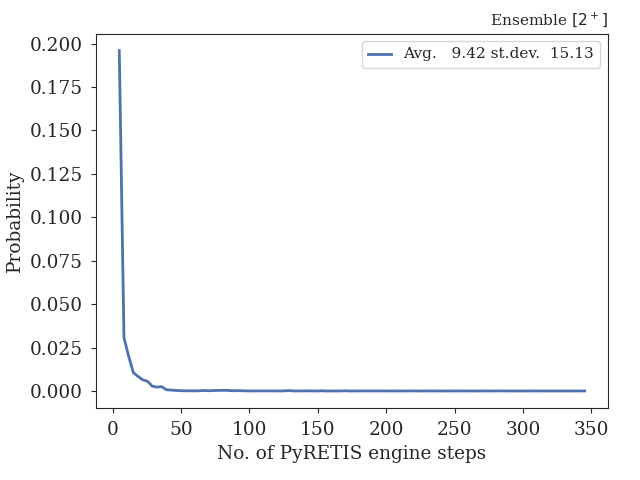
\includegraphics[width=0.45\linewidth]{003_lpath.png}%
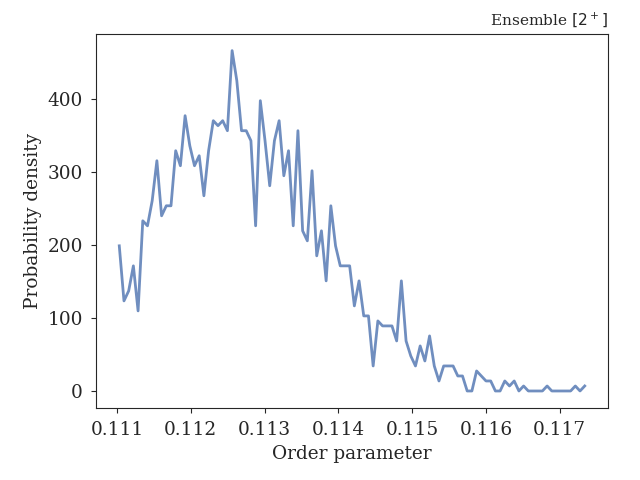
\includegraphics[width=0.45\linewidth]{003_shoots.png}%
\end{center}

\begin{center}
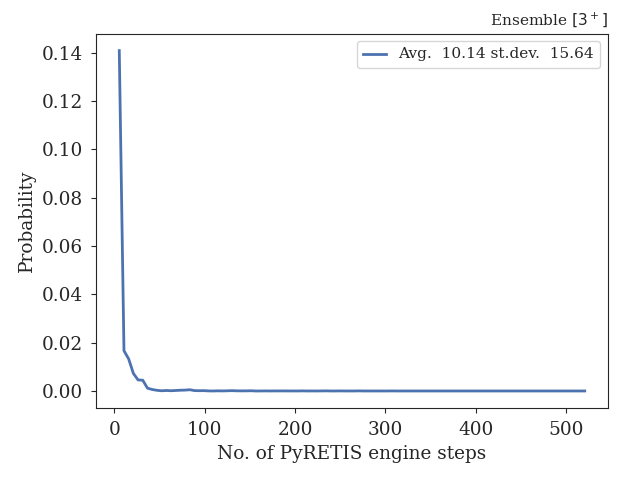
\includegraphics[width=0.45\linewidth]{004_lpath.png}%
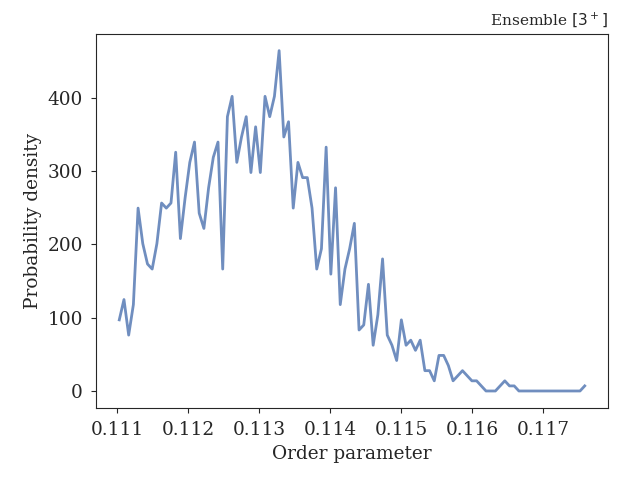
\includegraphics[width=0.45\linewidth]{004_shoots.png}%
\end{center}

\begin{center}
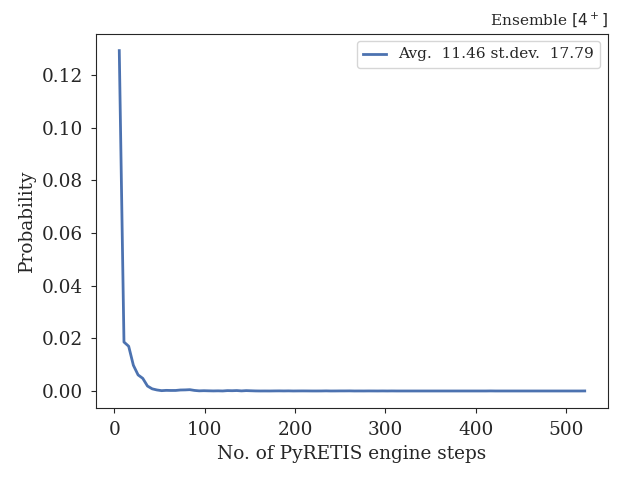
\includegraphics[width=0.45\linewidth]{005_lpath.png}%
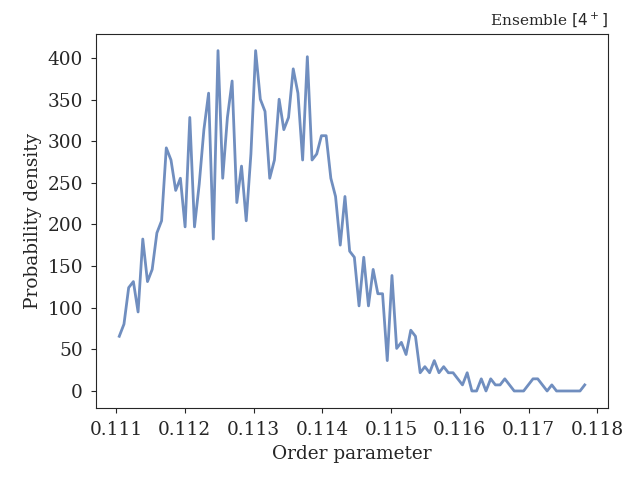
\includegraphics[width=0.45\linewidth]{005_shoots.png}%
\end{center}

\begin{center}
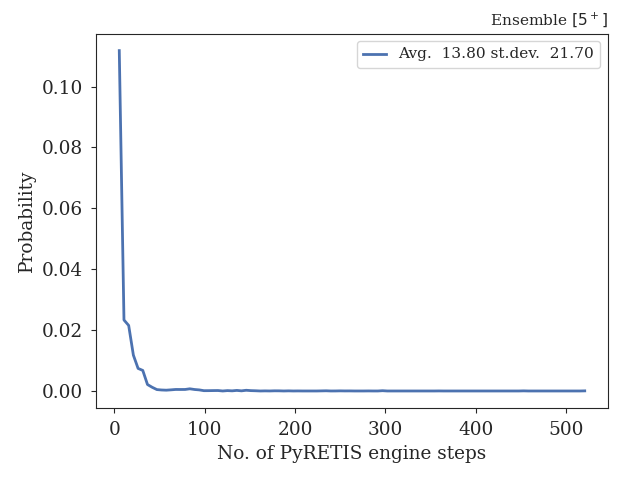
\includegraphics[width=0.45\linewidth]{006_lpath.png}%
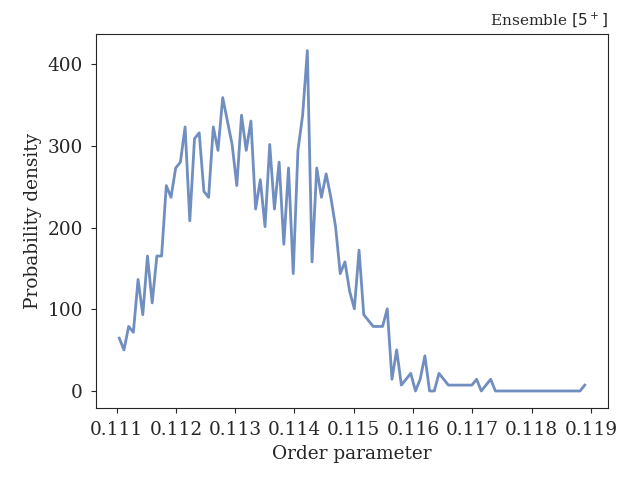
\includegraphics[width=0.45\linewidth]{006_shoots.png}%
\end{center}

\begin{center}
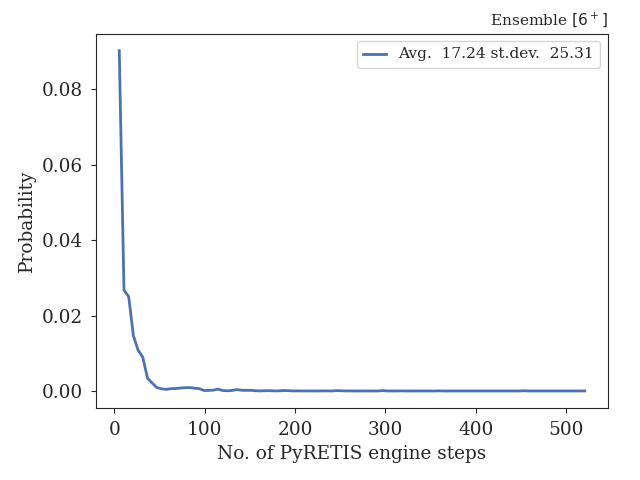
\includegraphics[width=0.45\linewidth]{007_lpath.png}%
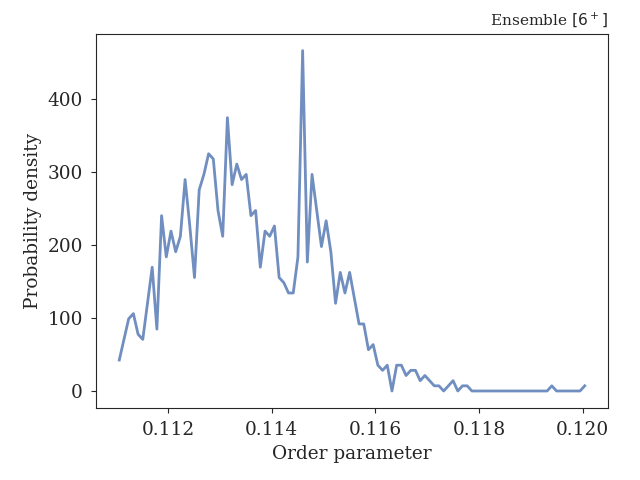
\includegraphics[width=0.45\linewidth]{007_shoots.png}%
\end{center}

\begin{center}
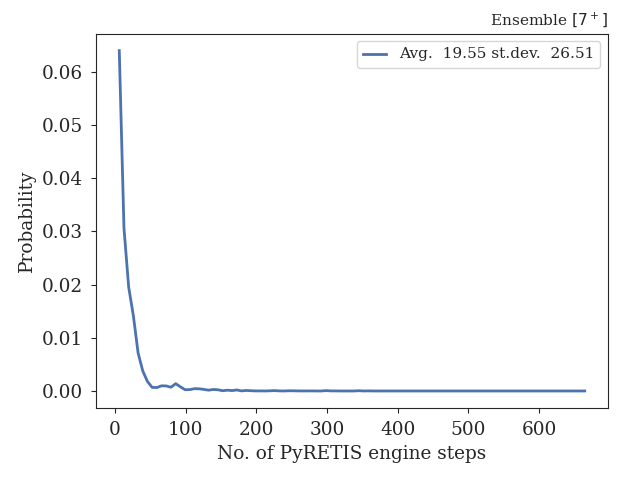
\includegraphics[width=0.45\linewidth]{008_lpath.png}%
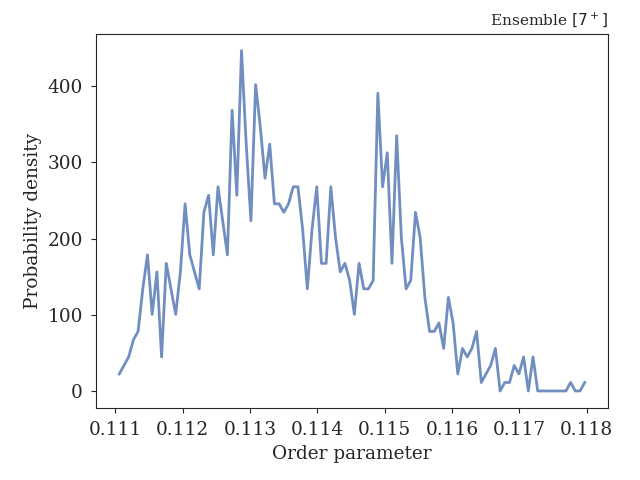
\includegraphics[width=0.45\linewidth]{008_shoots.png}%
\end{center}

\begin{center}
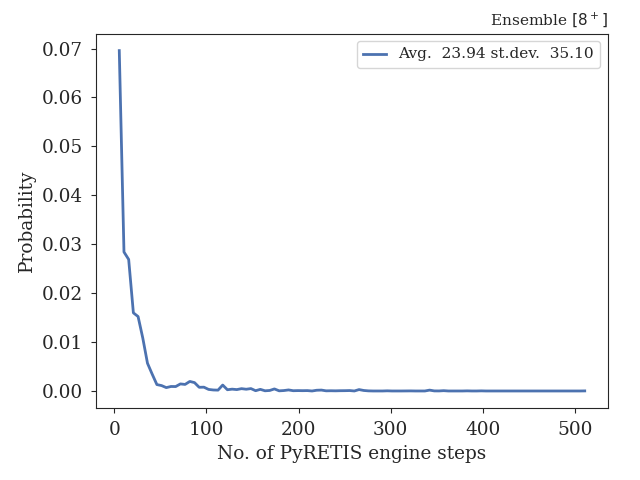
\includegraphics[width=0.45\linewidth]{009_lpath.png}%
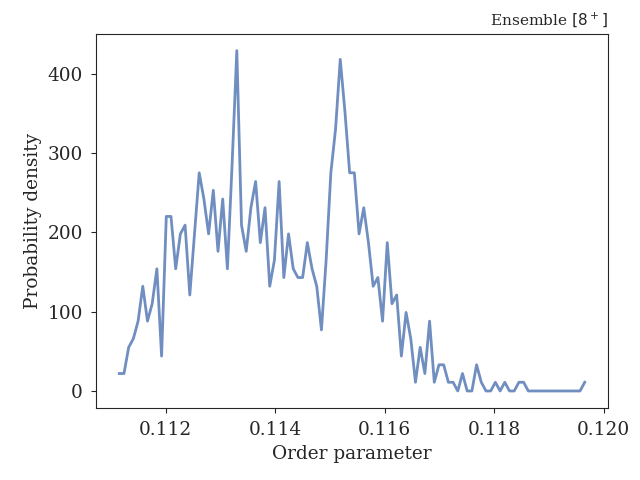
\includegraphics[width=0.45\linewidth]{009_shoots.png}%
\end{center}

\begin{center}
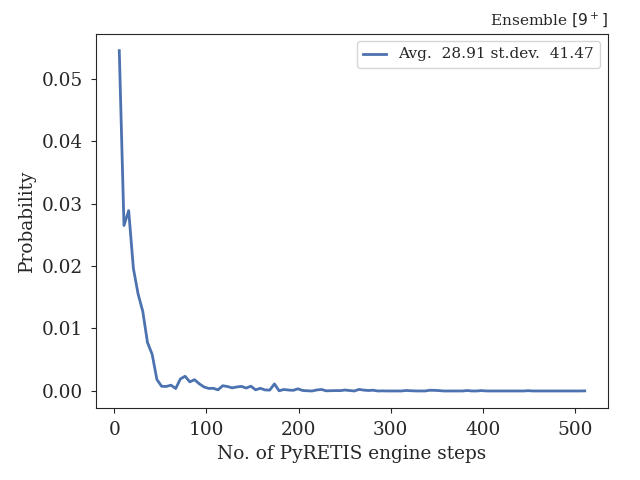
\includegraphics[width=0.45\linewidth]{010_lpath.png}%
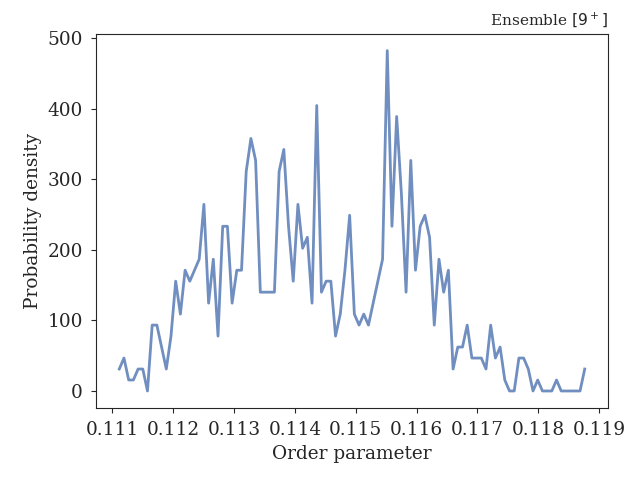
\includegraphics[width=0.45\linewidth]{010_shoots.png}%
\end{center}

\begin{center}
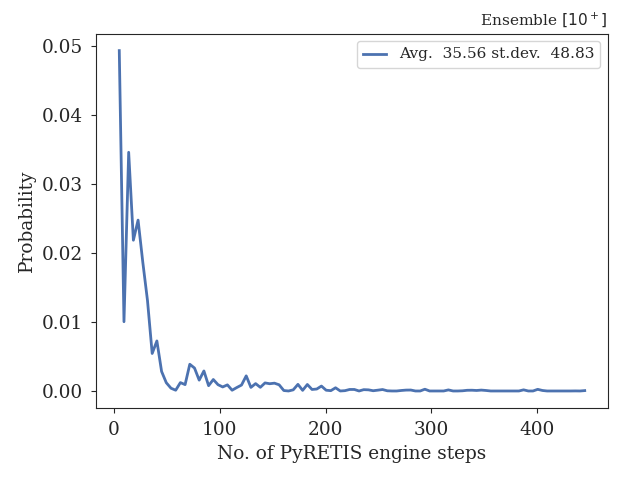
\includegraphics[width=0.45\linewidth]{011_lpath.png}%
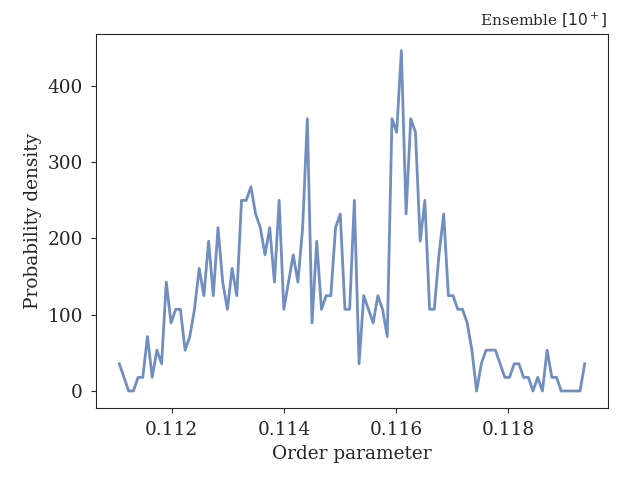
\includegraphics[width=0.45\linewidth]{011_shoots.png}%
\end{center}

\begin{center}
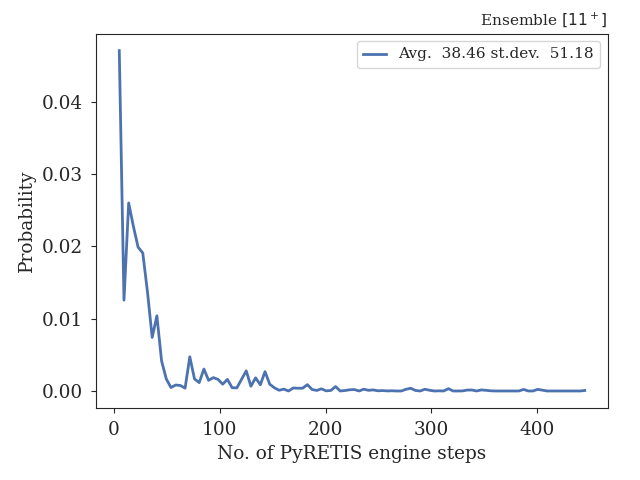
\includegraphics[width=0.45\linewidth]{012_lpath.png}%
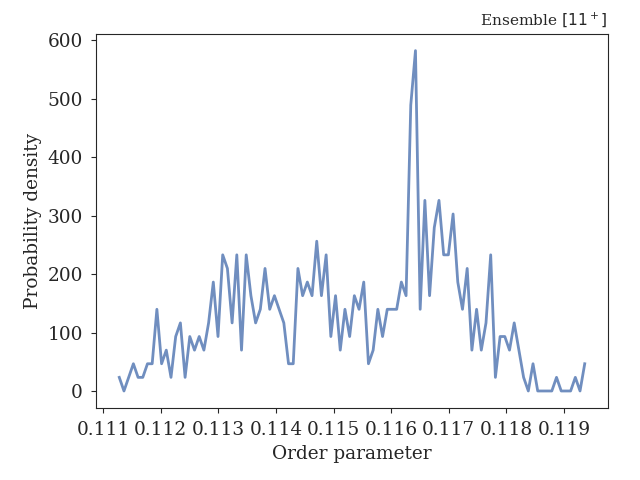
\includegraphics[width=0.45\linewidth]{012_shoots.png}%
\end{center}

\begin{center}
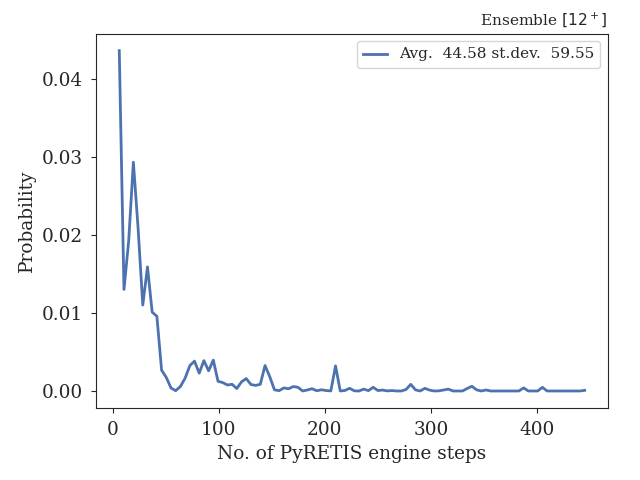
\includegraphics[width=0.45\linewidth]{013_lpath.png}%
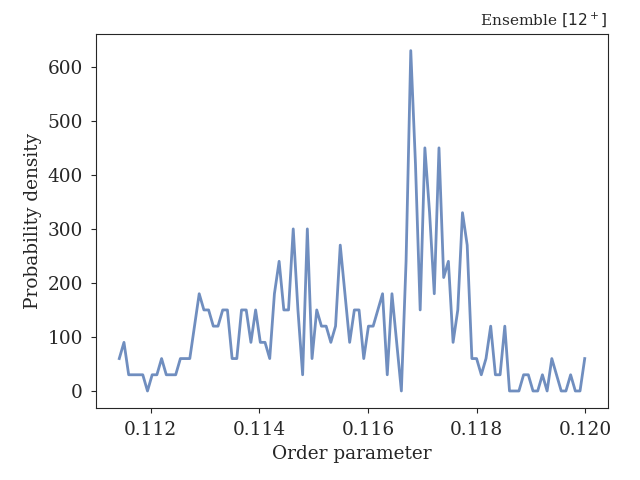
\includegraphics[width=0.45\linewidth]{013_shoots.png}%
\end{center}

\begin{center}
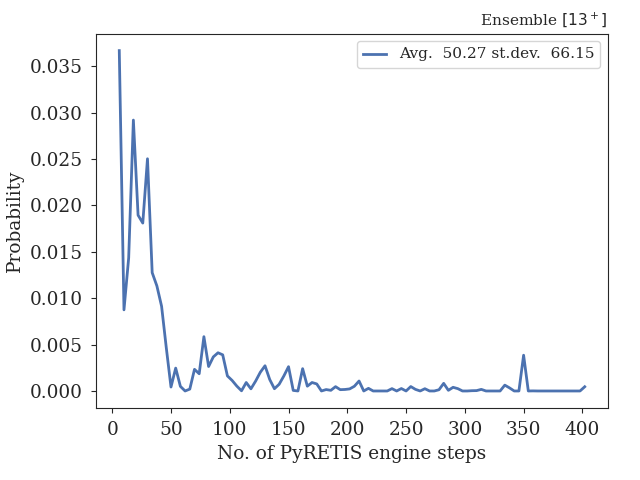
\includegraphics[width=0.45\linewidth]{014_lpath.png}%
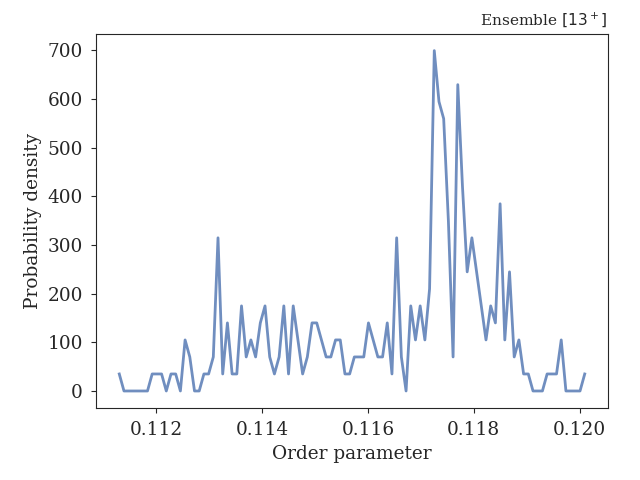
\includegraphics[width=0.45\linewidth]{014_shoots.png}%
\end{center}

\begin{center}
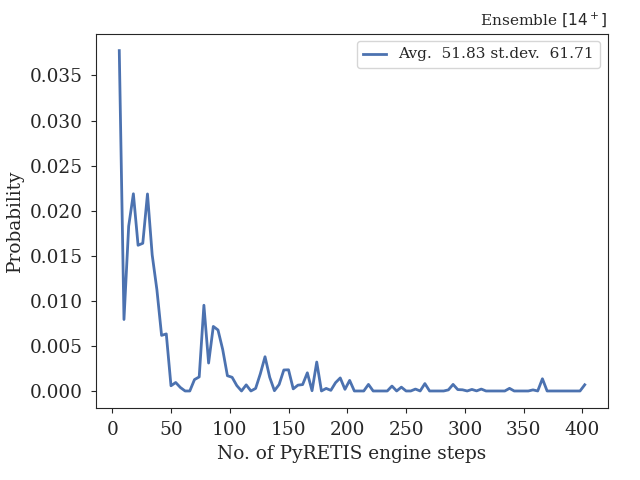
\includegraphics[width=0.45\linewidth]{015_lpath.png}%
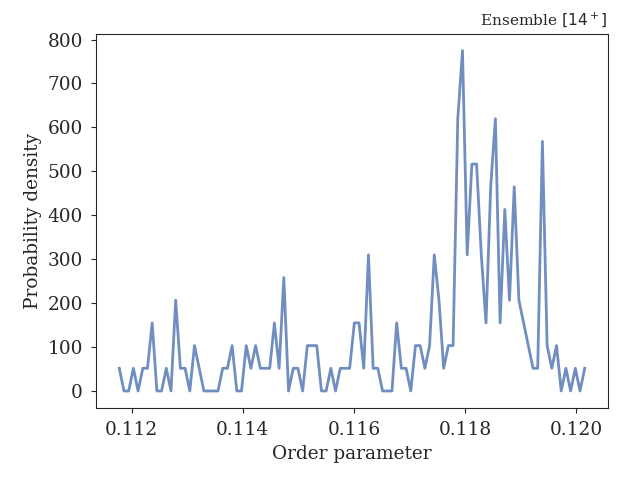
\includegraphics[width=0.45\linewidth]{015_shoots.png}%
\end{center}

\begin{center}
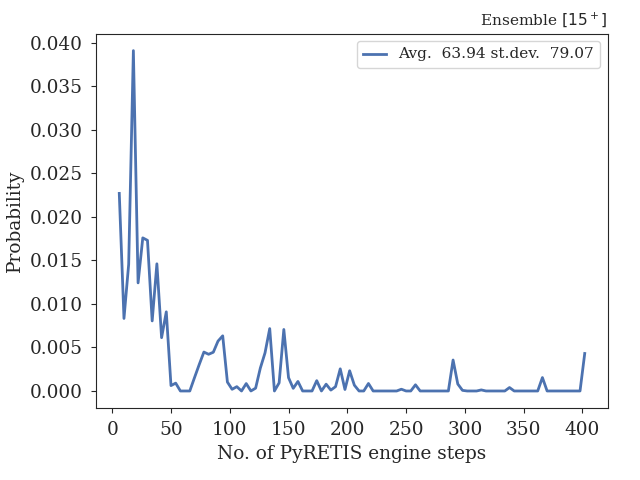
\includegraphics[width=0.45\linewidth]{016_lpath.png}%
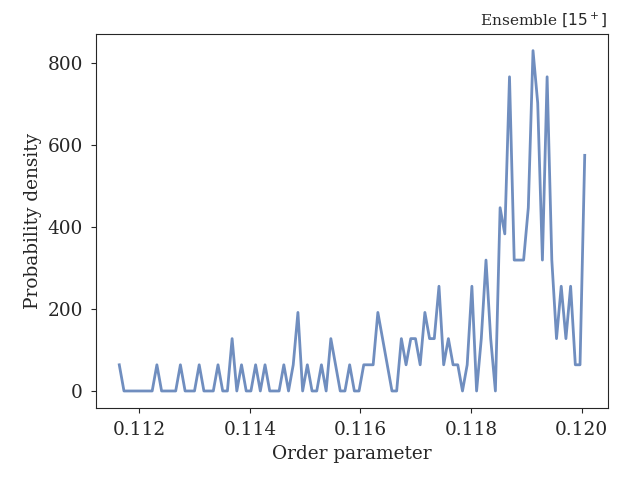
\includegraphics[width=0.45\linewidth]{016_shoots.png}%
\end{center}

\begin{center}
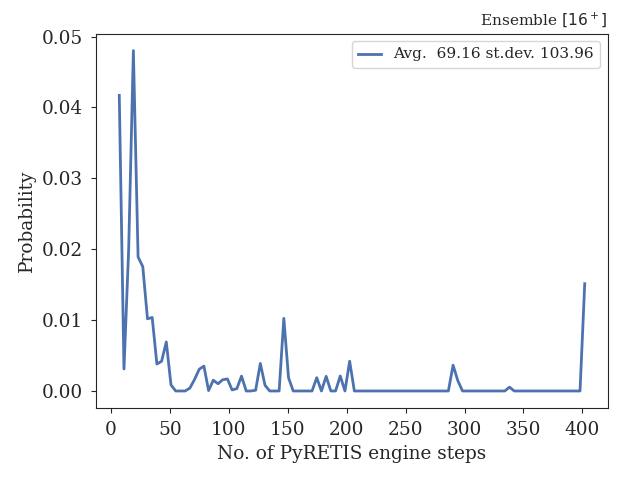
\includegraphics[width=0.45\linewidth]{017_lpath.png}%
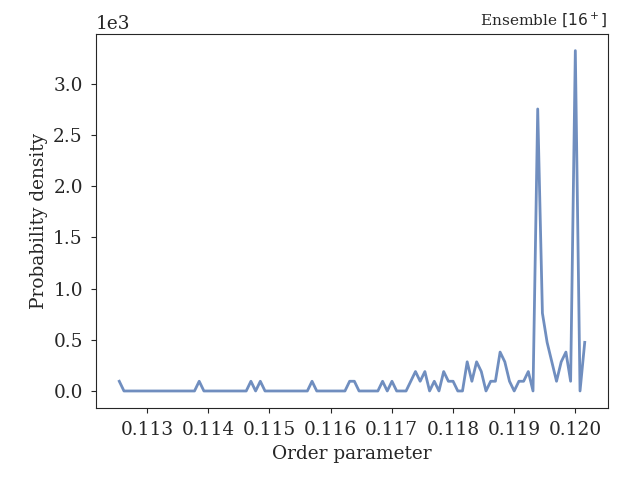
\includegraphics[width=0.45\linewidth]{017_shoots.png}%
\end{center}

\clearpage

\end{document}